\def\layersep{2.5cm}
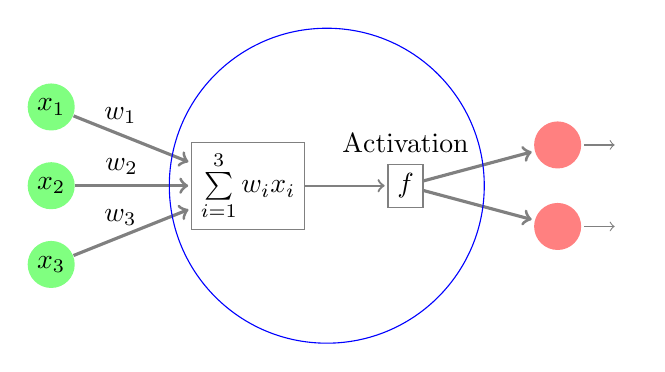
\begin{tikzpicture}[shorten >=1pt,->,draw=black!50, node distance=\layersep]
    \tikzstyle{neuron}=[circle,fill=black!25,minimum size=17pt,inner sep=0pt]
    \tikzstyle{input neuron}=[neuron, fill=green!50];
    \tikzstyle{output neuron}=[neuron, fill=red!50];
    \tikzstyle{every pin edge}=[<-,shorten <=1pt]
    \path
    % Summation
    (0,0)     node[draw] (summation) {$\sum\limits_{i=1}^{3} w_{i}x_{i}$}

    % Input nodes
    +(-2.5,1.0)  node[input neuron]  (input1) {$x_{1}$}
    +(-2.5,0)    node[input neuron]  (input2) {$x_{2}$}
    +(-2.5,-1.0) node[input neuron]  (input3) {$x_{3}$}

    % Activation function
    (2,0)    node[draw] (activation) {$f$} node[above=3mm]{Activation}

    % Output nodes
    +(15:2.0)  node[output neuron, pin={[pin edge={->}]right:}]  (output1) {}
    +(-15:2.0) node[output neuron, pin={[pin edge={->}]right:}]  (output2) {};

    % Link the different parts of the graph
    \draw[->,thick] (summation)--(activation);
    \draw[->,line width=0.4mm] (activation)--(output1) node[pos=.6,above]{};
    \draw[->,line width=0.4mm] (activation)--(output2) node[pos=.6,below]{};
    \draw[->,line width=0.4mm] (input1)--(summation) node[pos=.4,above]{$w_{1}$};
    \draw[->,line width=0.4mm] (input2)--(summation) node[pos=.4,above]{$w_{2}$};
    \draw[->,line width=0.4mm] (input3)--(summation) node[pos=.4,above]{$w_{3}$};
    \draw[blue] (1,0) circle(2);
\end{tikzpicture}